\chapter{Уламжлал}

\section{Өөрчлөлтийн харьцаа ба шүргэгч шулуун}

\begin{definition}[Өөрчлөлтийн харьцаа]
$a,b$ нь $a\ne b$ тогтмол тоонууд байг. $y=f(x)$ функцийг $x=a$-аас $x=b$ хүртэл өөрчлөхөд
\[
\Delta x=b-a,\qquad \Delta y=f(b)-f(a),
\]
\[
\frac{\Delta y}{\Delta x}=\frac{f(b)-f(a)}{b-a}
\]
-ийг $f(x)$ функцийн $[a,b]$ дээрх өөрчлөлтийн харьцаа гэнэ. Энэ нь $A(a,f(a))$ ба $B(b,f(b))$ цэгүүдийг дайрсан шулууны налалт юм.
\end{definition}

\begin{example}
$f(x)=x^2$ функцийн хувьд
\begin{enumerate}
  \item $x=-1$-ээс $x=2$ хүртэл: $\dfrac{\Delta y}{\Delta x}=\dfrac{2^2-(-1)^2}{2-(-1)}=\dfrac{3}{3}=1$.
  \item $x=a$-аас $x=a+h$ хүртэл: $\dfrac{(a+h)^2-a^2}{h}=2a+h$.
\end{enumerate}
\end{example}
\section{Уламжлалын тодорхойлолт ба тэмдэглэгээ}

\begin{definition}[Цэг дээрх уламжлал]
$f$ функц $x=a$ цэгийн орчимд тодорхойлогдсон байг. Хэрэв
\[
\lim_{h\to 0}\frac{f(a+h)-f(a)}{h}
\]
хязгаар оршин байвал $f$ функцийг нь $x=a$ цэг дээр \textbf{цэг дээр дифференциалчлагдах} функц гэнэ. Энэ хязгаарын утгийг $f$ функцийн $a$ цэг дээрх уламжлал гээд $f'(a)$ гэж тэмдэглэнэ.
\end{definition}

\begin{note}
$x=a$ цэг дээрх уламжлал $f'(a)$ нь $A(a,f(a))$ цэг дээр татсан шүргэгч шулууны налалт бөгөөд шүргэгч шулууны тэгшитгэл
\[
y - f(a) = f'(a)\,(x-a).
\] байдаг.
\end{note}

\begin{example}
$f(x)=x^2-2x-1$ үед
\[
f'(3)=\lim_{h\to 0}\frac{f(3+h)-f(3)}{h}
=\lim_{h\to 0}\frac{(3+h)^2-2(3+h)-1 - (9-6-1)}{h}=4.
\]
\end{example}

\begin{center}
\begin{tikzpicture}[scale=1]
  % Axes
  \draw[->] (-1,0) -- (5,0) node[right] {$x$};
  \draw[->] (0,-4) -- (0,6) node[above] {$y$};

  % f(x)=x^2-2x-1
  \draw[thick] plot[samples=200,domain=-0.2:4.5] (\x,{(\x*\x - 2*\x - 1)}) node[right] {$y=f(x)=x^2-2x-1$};

  % a=3 point
  \coordinate (P) at (3,{(3*3 - 2*3 - 1)});
  \fill (P) circle (2pt) node[above right] {$A(3,f(3))$};

  % tangent at x=3: f'(x)=2x-2 => f'(3)=4 ; y - f(3)=4(x-3)
  \draw[very thick,red] (1,{2+4*(1-3)}) -- (4.5,{2+4*(4.5-3)}) node[above right] {шүргэгч};

  % A few secants approaching tangent: pick b=3+h
  \foreach \h/\col in {1/blue,0.5/blue,0.25/blue}{
    \coordinate (B) at ({3+\h},{(3+\h)*(3+\h)-2*(3+\h)-1});
    \draw[\col] (P) -- (B);
    \fill (B) circle (1.5pt);
  }
\end{tikzpicture}
\end{center}

\subsection*{Тэмдэглэгээ}
$y=f(x)$ бол түүний $a$ цэг дээрх уламжлалыг $f'(a)$, $\dfrac{dy}{dx}(a)$, $Df(a)$, $y'(a)$ зэрэг тэмдэглэнэ.
\section{Хялбар функцүүдийн цэг дээрх уламжлал}

\begin{example}
Дараах функцийг тодорхойлолтын дагуу бодож $x=a$ цэг дээрх уламжлалыг ол.
\begin{enumerate}
  \item $f(x)=c$ (тогтмол функц).  
  \[
  f'(a)=\lim_{h\to0}\frac{c-c}{h}=0.
  \]
  Тэгэхээр тогтмол функцийн цэг дээрх уламжлал $0$.
  
  \item $f(x)=x$.  
  \[
  f'(a)=\lim_{h\to0}\frac{(a+h)-a}{h}=\lim_{h\to0}1=1.
  \]
  Иймээс $y=x$ шулууны бүх цэг дээрх уламжлал $1$, өөрөөр хэлбэл шүргэгчийн налалт тогтмол.
  
  \item $f(x)=x^2$.  
  \[
  f'(a)=\lim_{h\to0}\frac{(a+h)^2-a^2}{h}=\lim_{h\to0}\frac{2ah+h^2}{h}=2a.
  \]
\end{enumerate}
\end{example}
\section{Дифференциалчлах дүрмүүд}

\begin{theorem}[Арифметик үйлдлүүд ба уламжлалын дүрмүүд]
$f,g$ дифференциалчлагддаг функцүүд ба  $c$ тогтмол тоо бол
\begin{enumerate}
    \item $(c\cdot f)'(a)=c\cdot f'(a)$
    \item $(f\pm g)'(a)=f'(a)\pm g'(a)$
    \item $(fg)'(a)=f'(a)g(a)+f(a)g'(a)$
    \item $
\left(\frac{f}{g}\right)'(a)=\frac{f'(a)g(a) - f(a)g'(a)}{g^2(a)}\quad (g(a)\ne 0)$
\end{enumerate}
байна.
\end{theorem}

\begin{example}
\begin{enumerate}
  \item $y=3x^2 \;\Rightarrow\; y'=6x$.
  \item $y=x^3+\tfrac12x^2-3x+4 \;\Rightarrow\; y'=3x^2+x-3$.
  \item $y=(x^2-1)(2x^2+x-3) \;\Rightarrow\; y'=8x^3+3x^2-10x-1$.
  \item $y=\dfrac{1}{x} \;\Rightarrow\; y'= -\dfrac{1}{x^{2}}$.
  \item $y=\dfrac{3x-2}{2x+1} \;\Rightarrow\; y'=\dfrac{7}{(2x+1)^2}$.
  \item $y=\sqrt{x}$. \textit{Бодолт:} $f(x)=\sqrt{x}$ гэж тавья. Тэгвэл
        $f(x)\cdot f(x)=x$. Уржвэрийн дүрмээр уламжлал авбал
        \[
           2\,f(x)\,f'(x) \;=\; 1
           \quad\Longrightarrow\quad
           f'(x) \;=\; \frac{1}{2\,f(x)} \;=\; \frac{1}{2\sqrt{x}}.
        \]
        Иймээс $y'=\dfrac{1}{2\sqrt{x}}$.
\end{enumerate}
\end{example}

\begin{definition}[Уламжлалын функц]
Хэрэв $f(x)$ функц нь тодорхойлогдох мужийнхаа \emph{бүх цэг дээр} уламжлалтай бол 
тэрхүү цэг $x$ бүрт $f'(x)$ тоог харгалзуулах функцийг $f$-ийн уламжлалын функц гэнэ.  

Өөрөөр хэлбэл, хэрэв $f$ нь муж $D$-ийн бүх цэг дээр уламжлалтай бол  
\[
g:D\to\mathbb{R}, \qquad g: x\to f'(x)
\]
функцийг $f$-ийн уламжлалын функц гэж нэрлээд $g(x)=f'(x)$ гэнэ.
\end{definition}
\section{Тасралтгүй ба дифференциалчлагдах чанар}

\begin{theorem}
$f$ функц $x=a$ цэг дээр дифференциалчлагдвал $f$ нь $x=a$ цэг дээр тасралтгүй.
\end{theorem}

\begin{prof}
$h=x-a$ гэе. Тэгвэл
\[
\lim_{x\to a} \big(f(x)-f(a)\big)=\lim_{h\to 0}\frac{f(a+h)-f(a)}{h}\cdot h
= f'(a)\cdot 0=0.
\]
Иймээс $\displaystyle \lim_{x\to a}f(x)=f(a)$ буюу $f$ нь цэг дээр тасралтгүй.
\end{prof}

\begin{example}[Тасралттай боловч дифференциалчлагдахгүй функц]
\begin{enumerate}
  \item $f(x)=|x|$ байг. $\displaystyle \lim_{h\to 0^+}\frac{|h|}{h}=1$, $\displaystyle \lim_{h\to 0^-}\frac{|h|}{h}=-1$ тул $x=0$ цэг дээрх уламжлал оршихгүй.
  \item $f(x)=\sqrt{|x|}$: $\displaystyle \lim_{h\to 0^+}\frac{\sqrt{|h|}}{h}=+\infty$, $\displaystyle \lim_{h\to 0^-}\frac{\sqrt{|h|}}{h}=-\infty$ — шүргэгч босоо.
\end{enumerate}
\end{example}

\begin{center}
\begin{tikzpicture}[scale=1.0]
  % Axes
  \draw[->] (-3,0) -- (3,0) node[right] {$x$};
  \draw[->] (0,-0.5) -- (0,3.2) node[above] {$y$};

  % |x|
  \draw[thick] plot[samples=200,domain=-2.5:2.5] (\x,{abs(\x)}) node[right] {$y=|x|$};
  % One-sided slopes annotation
  \draw[red,very thick] (-2,-2) -- (0,0);
  \draw[red,very thick] (0,0) -- (2,2);
  \fill (0,0) circle (2pt) node[below left] {$x=0$};

  \node[below] at (-1.2,-0.2) {налалт $-1$};
  \node[above] at (1.2,1.4) {налалт $+1$};
\end{tikzpicture}
\hspace{1cm}
\begin{tikzpicture}[scale=1.0]
  % Axes
  \draw[->] (-3,0) -- (3,0) node[right] {$x$};
  \draw[->] (0,-0.5) -- (0,2.8) node[above] {$y$};

  % sqrt(|x|)
  \draw[thick,domain=0:2.8,samples=200] plot (\x,{sqrt(\x)}) node[right] {$y=\sqrt{|x|}$};
  \draw[thick,domain=-2.8:0,samples=200] plot (\x,{sqrt(abs(\x))});

  % Vertical tangent indication
  \draw[red,very thick] (0,0) -- (0,2.2) node[above] {босоо шүргэгч};
  \fill (0,0) circle (2pt) node[below left] {$x=0$};
\end{tikzpicture}
\end{center}
\section{Тригонометр, илтгэгч ба логарифм функцийн уламжлал}

\begin{theorem}[Тригонометр функцийн уламжлал]
\[
(\sin x)' = \cos x, \qquad (\cos x)' = -\sin x
\]
\end{theorem}
\begin{prof}
\begin{enumerate}
  \item  
  Тодорхойлолтоор:
  \[
  \lim_{h\to0}\frac{\sin(x+h)-\sin x}{h}
  =\lim_{h\to0}\frac{\sin x\cos h+\cos x\sin h-\sin x}{h}
  =\lim_{h\to0}\big(\sin x\frac{\cos h-1}{h}+\cos x\frac{\sin h}{h}\big).
  \]
  $\displaystyle \lim_{h\to0}\frac{\cos h-1}{h}=0$ ба $\displaystyle \lim_{h\to0}\frac{\sin h}{h}=1$ тул:
  \[
  (\sin x)'=\cos x.
  \]

  \item $(\cos x)'=-\sin x$.  
  $$
  \lim_{h\to0}\frac{\cos(x+h)-\cos x}{h}
  =\lim_{h\to0}\frac{\cos x\cos h-\sin x\sin h-\cos x}{h}
  =$$
  $$\lim_{h\to0}\big(\cos x\frac{\cos h-1}{h}-\sin x\frac{\sin h}{h}\big)
  =-\sin x.
  $$
\end{enumerate}
\end{prof}
\begin{example}
\begin{enumerate}
  \item $y=\sin 2x \;\Rightarrow\; y'=(2\sin x\cos x)'=2(\cos x\cos x+\sin x(-\sin x))=2\cos 2x.$
  \item $y=\tan x=\dfrac{\sin x}{\cos x} 
  \;\Rightarrow\; y'=\dfrac{\cos^2 x+\sin^2 x}{\cos^2 x}
  =\dfrac{1}{\cos^2 x}.$
\end{enumerate}
\end{example}

\begin{center}
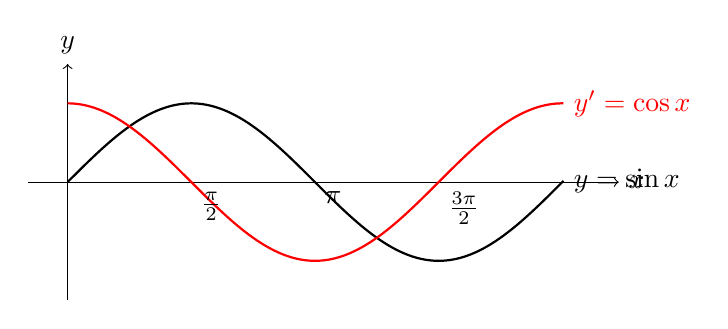
\begin{tikzpicture}[scale=1]
  \draw[->] (-0.5,0) -- (7,0) node[right] {$x$};
  \draw[->] (0,-1.5) -- (0,1.5) node[above] {$y$};
  \draw[thick,domain=0:6.3,samples=200] plot(\x,{sin(\x r)}) node[right] {$y=\sin x$};
  \draw[red,thick,domain=0:6.3,samples=200] plot(\x,{cos(\x r)}) node[right] {$y'=\cos x$};
  \node[below right] at (1.57,0) {$\frac{\pi}{2}$};
  \node[below right] at (3.14,0) {$\pi$};
  \node[below right] at (4.71,0) {$\frac{3\pi}{2}$};
\end{tikzpicture}
\end{center}

\section{Илтгэгч ба урвуу функцийн уламжлал}

\subsection*{Илтгэгч функцийн уламжлал ба хэрэглээ}

\begin{theorem}[Илтгэгч функцийн уламжлал]
\[
(e^x)' = e^x.
\]
\end{theorem}

\begin{prof}
Тодорхойлолтоор:
\[
(e^x)' = \lim_{h\to 0} \frac{e^{x+h} - e^x}{h}
= e^x \lim_{h\to 0}\frac{e^h - 1}{h}.
\]
Хязгаар $\displaystyle \lim_{h\to 0}\frac{e^h - 1}{h}=1$ тул $(e^x)'=e^x$.
\end{prof}

\begin{example}
\begin{enumerate}
  \item $y=e^{2x}$ бол :
  \[
  y' = (e^{2x})'=(e^x\cdot e^x)'=e^x\cdot e^x+e^x\cdot e^x = 2e^{2x}.
  \]
  \item $y=e^{-x}$ бол
  \[
  y' = (e^{-x})'=\left(\dfrac{1}{e^x}\right)'=\dfrac{1'\cdot e^x-1\cdot (e^x)'}{(e^x)^2}= -e^{-x}.
  \]
\end{enumerate}
\end{example}
\begin{theorem}[Давхар функцийн уламжлал]
Хэрэв $y=g(x)$ функц нь $x=a$ цэг дээр дифференциалчлагддаг, $y=f(x)$ нь $x=g(a)$ цэг дээр дифференциалчлагддаг бол $y=f(g(x))$ функц $x=a$ цэг дээр дифференциалчлагдах ба
\[
\boxed{\frac{dy}{dx}(a) = \frac{dy}{du}(a)\cdot\frac{du}{dx}(a)}.
\] байна.
\end{theorem}

\begin{example}
\begin{enumerate}
  \item $y=a^x=e^{x\ln a}$ тул $(a>0, a\ne1)$ үед:
  \[
  y' = e^{x\ln a}\cdot \ln a = a^x \ln a.
  \]
  \item $y=\sin(e^x)$:
  \[
  y' = \cos(e^x)\cdot e^x.
  \]
  \item $y=e^{\sin x}$:
  \[
  y' = e^{\sin x}\cdot \cos x.
  \]
  \item $y=\sqrt{1+e^{2x}}$:
  \[
  y'=\frac{1}{2\sqrt{1+e^{2x}}}\cdot 2e^{2x}\cdot 1
  =\frac{e^{2x}}{\sqrt{1+e^{2x}}}.
  \]
\end{enumerate}
\end{example}

\begin{theorem}[Урвуу функцийн уламжлалын теорем]
Урвуутай функц $y=f(x)$ нь $x=a$ цэг дээр уламжлалттай, $f(a)=b$ утгатай, $f'(a)\neq0$ гэж бодъё. Тэгвэл $y=f(x)$-ийн урвуу функц $y=f^{-1}(x)$ нь $x=b$ цэг дээр дифференциалчлагдах ба 
\[
\boxed{(f^{-1})'(b) = \dfrac{1}{f'(a)}=\dfrac{1}{f'(f^{-1}(b))}}
\] байна.
\end{theorem}
\begin{example}
\begin{enumerate}
  \item $y=\ln x$ бол $x=e^y$. Урвуу функцийн дүрмээр:
  \[
  \frac{dy}{dx} = \frac{1}{\frac{dx}{dy}} = \frac{1}{e^y} = \frac{1}{x}.
  \]
  \item $y=\arcsin x$ бол $\sin y = x$. Дифференциал авбал:
  \[
  \cos y \, \frac{dy}{dx} = 1
  \quad \Longrightarrow \quad
  \frac{dy}{dx} = \frac{1}{\cos y}.
  \]
  Харин $\cos y = \sqrt{1-\sin^2 y}=\sqrt{1-x^2}$ тул:
  \[
  (\arcsin x)' = \frac{1}{\sqrt{1-x^2}}.
  \]
  \item $y=\arctan x$: $\tan y = x$ тул $\sec^2 y\,\dfrac{dy}{dx}=1$ буюу
  \[
  (\arctan x)'=\cos^2 y=\frac{1}{1+\tan^2 y}=\frac{1}{1+x^2}.
  \]
\end{enumerate}
\end{example}
\newpage
\section{Уламжлал бодох техник}

\subsection*{1. Уламжлалын жагсаалт}
\begin{enumerate}
  \item $(c)'=0$ — тогтмол функцийн уламжлал $0$.
  \item $(x)'=1$ , $y=x$ функцийн уламжлал $1$.
  \item $(x^{a})'=ax^{a-1}$ \;($a\in\mathbb{R}$).
  \item $(e^x)'=e^x$, \; $(a^x)'=a^x\ln a$.
  \item $(\ln x)'=\dfrac{1}{x}$.
  \item $(\sin x)'=\cos x$, \; $(\cos x)'=-\sin x$, \; $(\tan x)'=\dfrac{1}{\cos^2 x}$.
  \item $(cf)'=cf'$, \; $(f\pm g)'=f'\pm g'$, \; $(fg)'=f'g+fg'$, \;
  $\displaystyle \left(\dfrac{f}{g}\right)'=\dfrac{f'g-fg'}{g^2}$.
  \item \textbf{Гинжин дүрэм:} $(f(g(x)))'=f'(g(x))\cdot g'(x)$.
\end{enumerate}


\subsection*{2. Бодлого бодох жор}
\begin{itemize}
  \item \textbf{Эхлээд} логgарифм, илтгэгч, зэрэг, тригнометр—аль дүрэм хэрэглэхийг тодорхойл.
  \item \textbf{Дараа нь} үржвэр/ногдвор/гинжин аль нь давамгайлж буйг тогтоож, \textbf{давхар} хэрэглэж эвлүүл.
  \item \textbf{Хялбарчлах хувиргалт} (триг $=\dfrac{\sin}{\cos}$, $\ln\sqrt{\ }=\tfrac12\ln$ гэх мэт) хийж хялбарчил.
\end{itemize}

\subsection*{3. Хялбар жишээнүүд}
\begin{example}
\begin{enumerate}
  \item $y=\dfrac{\sin x}{x}$.\; $y'=\dfrac{x\cos x-\sin x}{x^2}$.
  \item $y=e^{2x-3}$.\; $y'=2e^{2x-3}$.
  \item $y=\ln(\sqrt{1+x^2})$.\; $y'=\dfrac{x}{1+x^2}$ \; (гинжин + $\ln\sqrt{\ }=\tfrac12\ln$).
  \item $y=\sin(e^x)$.\; $y'=\cos(e^x)\cdot e^x$.
  \item $y=(x^2+1)^{5}$.\; $y'=5(x^2+1)^{4}\cdot 2x=10x(x^2+1)^4$.
\end{enumerate}
\end{example}

\subsection*{4.Далд функцийн уламжлал}
\begin{definition}
$F(x,y)=0$ тэгшитгэлийнхэлбэрийн хамаарлыг $y=y(x)$ гэж үзээд $x$-ийн хувьд дифференциалчлахыг \emph{имплицит уламжлал} гэнэ.
\end{definition}

\begin{example}
Тойрог: $x^2+y^2=25$. $x$-ийн хувьд дифференциалчилбал $2x+2y\,y'=0 \Rightarrow y'=-\dfrac{x}{y}$.
\end{example}

\begin{example}
$xy+\sin y = x^2$. Дифференциалчилбал
\[
y + x\,y' + \cos y \cdot y' = 2x 
\;\;\Rightarrow\;\;
y'(x+\cos y)=2x-y
\;\;\Rightarrow\;\;
\boxed{y'=\dfrac{2x-y}{\,x+\cos y\,}}.
\]
\end{example}

\subsection*{5. Логарифмын уламжлал (Зэрэгт-илтгэгч функц)}
\begin{remark}
$y>0$ үед $\ln y$ авч, тэгшитгэлийг логарифмдан хоёр талд нь дифференциалчлах аргыг \emph{логарифмын уламжлал} гэдэг.
\end{remark}

\begin{example}
$y=x^x$ ($x>0$). $\ln y = x\ln x \Rightarrow \dfrac{y'}{y}=\ln x + 1 \Rightarrow \boxed{y'=x^x(\ln x + 1)}$.
\end{example}

\begin{example}
$y=(x^2+1)^x$ ($x>0$). $\ln y = x\ln(x^2+1)\Rightarrow \dfrac{y'}{y}=\ln(x^2+1)+\dfrac{2x^2}{x^2+1}$.\\
Иймд $\boxed{y'=(x^2+1)^x\!\left[\ln(x^2+1)+\dfrac{2x^2}{x^2+1}\right]}$.
\end{example}

\subsection*{6. $\boldsymbol{a^x}$ ба $\boldsymbol{\log}$–ын \emph{хэрэглээ} }
\begin{example}
\begin{enumerate}
  \item $y=a^x$ ($a>0,a\ne1$). $y'=a^x\ln a$. \;
        Ж: $y=2^{3x}$ бол $y'=3\ln2\cdot 2^{3x}$.
  \item $y=\dfrac{\ln x}{x^2}$.\; $y'=\dfrac{1}{x}\cdot\dfrac{1}{x^2} + \ln x \cdot \left(-\dfrac{2}{x^3}\right)=\dfrac{1-2\ln x}{x^3}$.
  \item $y=e^{\sqrt{x}}$.\; $y'=e^{\sqrt{x}}\cdot\dfrac{1}{2\sqrt{x}}$.
  \item $y=\log_a(\sqrt{x})$.\; $y'=\dfrac{1}{x\ln a}\cdot\dfrac{1}{2}=\dfrac{1}{2x\ln a}$.
\end{enumerate}
\end{example}

\section{Семинар}
Дараах функцүүдийн уламжлалыг ол.
\begin{multicols}{2}
\begin{enumerate}
  \item $y=x^2-3x+1$ функцийн $x=2$ дээрх шүргэгч шулууны тэгшитгэлийг ол. Шүргэгчид перпенпдикуляр, шүргэлтийн цэгийг байрсан шулууны тэгшитгэл бич. Энэ шулуунийг нормал шулуун гэдэг.
 \item $y=\sqrt{x}$ функцийн $x=4$ дээрх шүргэгч ба нормал шулууны тэгшитгэлийг ол.
 \item Материал цэгийн хөдөлгөөн
\[
s(t)=t^3-6t^2+9t
\]
хуулиар өгөгдөв.  
а) Хурд $v(t)$-г ол.  
б) Хурдатгал $a(t)$-г ол.  
в) $t=2$ үед хурдыг ол.

 \item Материал цэгийн хөдөлгөөн
\[
s(t)=\sin t
\]
хуулиар өгөгдөв.  
а) Хурд $v(t)$-г ол.  
б) Хурдатгал $a(t)$-г ол.  
в) $t=\pi$ үед цэгийн хурдыг ол.
\item $y=x^2$ ба $y=x^2+4x+3$ муруйнуудын ерөнхий шүргэгч шулууныг ол.
  \item $y = 3x^2 - 5x + 1$
  \item $y = x^4 - \tfrac{1}{3}x^3 + 2.5x - 0.1$
  \item $y = \sqrt[3]{x} + 3\sqrt{2}$
  \item $y = \cos \tfrac{\pi}{3}$
  \item $y = \dfrac{x^2}{\sqrt{x}} - \sqrt{x}$
  \item $y = \dfrac{x^2 + 3x - 1}{x - 3}$
  \item $y = \dfrac{t^2 - 5t - 1}{t^3}$
  \item $y = (\sqrt{x} + 1)\left(\dfrac{1}{\sqrt{x}} - 1\right)$
  \item $y = (x^2 - 1)(x^2 - 4)(x^2 - 9)$
  \item $y = \dfrac{x + 1}{x - 1}$
  \item $y = \dfrac{x}{x^2 + 1}$
  \item $y = \dfrac{1 - x^3}{1 + x^3}$
  \item $y = \dfrac{1}{x + 2} - \dfrac{3}{x^2 + 1}$
  \item $y = \sin x + \cos x$
  \item $y = x \sin x + \cos x$
  \item $y = \tan x + \cot x$
  \item $y = \dfrac{x \sin x}{1 + \cos x}$
  \item $y = 2^x$
  \item $y = -\dfrac{1}{3^x}$
  \item $y = \dfrac{x}{4^x}$
  \item $y = e^x + x e$
  \item $y = -x^2 \log_2 x$
  \item $y = x \ln x$
  \item $y = \dfrac{1}{\ln x}$
  \item $y = -x \arctan x$
  \item $y = (\arctan x)^2$
  \item $y = \dfrac{\arccos x}{x}$
  \item $y = (1 + 2x)^{30}$
  \item $y = (1 - x^2)^{20}$
  \item $y = (5x^3 + x^2 - 4)^5$
  \item $y = \dfrac{1 + \sqrt{x}}{1 + \sqrt{2x}}$
  \item $y = 3 \sin(3x + 5)$
  \item $y = (x - a)(x - b)(x - c)(x - d)$
  \item $y = (x^2 + 1)^4$
  \item $y = (1 - x)^{20}$
  \item $y = (1 + 2x)^{30}$
  \item $y = (1 - x^2)^{10}$
  \item $y = (5x^3 + x^2 - 4)^5$
  \item $y = (x^3 - x)^6$
  \item $y = \left(7x^2 - \dfrac{4}{x} + 6\right)^6$
  \item $s = \left(t^3 - \dfrac{1}{t^3} + 3\right)^4$
  \item $y = \left(\dfrac{x+1}{x-1}\right)^2$
  \item $y = \left(\dfrac{1 + x^2}{1 + x}\right)^5$
  \item $y = (2x^3 + 3x^2 + 6x + 1)^4$
  \item $v = \dfrac{(s + 4)^2}{s + 8}$
  \item $s = -\dfrac{t^3}{(1 - t)^2}$
  \item $y = \dfrac{1 + \sqrt{x}}{1 + \sqrt{2x}}$
  \item $y = \dfrac{1 - \sqrt[3]{2x}}{1 + \sqrt[3]{2x}}$
  \item $y = \sqrt{1 - x^2}$
  \item $y = \left(1 - 2x^{1/2}\right)^4$
\end{enumerate}
\end{multicols}
\section{Гэрийн даалгавар: Уламжлал ол.}
\begin{multicols}{2}
\begin{enumerate}
  \item $y=\dfrac{1}{x}$ функцийн $x=1$ дээрх шүргэгч ба нормал  шулууны тэгшитгэлийг ол.
  \item $y=\sin x$ функцийн $x=\dfrac{\pi}{3}$ дээрх шүргэгч ба нормал шулууны тэгшитгэлийг ол.
  \item Материал цэгийн хөдөлгөөн
\[
s(t)=t^2+2t
\]
хуулиар өгөгдөв.  
а) Хурд $v(t)$-г ол.  
б) $t=1$ үед хурдыг ол.  
в) Ямар үед цэг зогсох вэ?
\item $y=x^2$ ба $y=-x^2-4$ муруйнуудын ерөнхий шүргэгч шулууныг ол.

  \item $y = (1 + \sqrt[3]{x})^3$
  \item $y = a \tan\!\left(\dfrac{x}{k} + b\right)$
  \item $y = \sqrt{1 + \sqrt{2px}}$
  \item $y = \arctan(x^2 - 3x + 2)$
  \item $y = \lg(x - \cos x)$
  \item $y = 3\cos^2 x - \cos^3 x$
  \item $y = 5\tan\dfrac{x}{5} + \tan\dfrac{\pi}{8}$
  \item $y = \dfrac{1}{\sqrt[3]{x + \sqrt{x}}}$
  \item $y = \sin\dfrac{x}{2}\sin2x$
  \item $y = \sin(e^{\cos x})$
  \item $y = x^5\sqrt[3]{x^6 - 8}$
  \item $y = e^{-x^2}\ln x$
  \item $y = \left(\sqrt{x} + \dfrac{1}{\sqrt{x}}\right)^{10}$
  \item $y = e^{2x+3}\!\left(x^2 - x + \dfrac{1}{2}\right)$
  \item $y = \dfrac{1}{\sqrt{3}}\arctan\dfrac{x\sqrt{3}}{1 - x^2}$
  \item $y = \dfrac{\tan\dfrac{x}{2} + \cot\dfrac{x}{2}}{x}$
  \item $y = \sin^2\dfrac{x}{3}\cot\dfrac{x}{2}$
  \item $y = \dfrac{\sqrt[5]{4x^6 + 2}}{3x^4}$
  \item $y = \ln\!\left(x + \sqrt{a^2 + x^2}\right)$
  \item $y = x \arctan\sqrt{x}$
  \item $y = \sqrt{1 + \tan^2 x + \tan^4 x}$
  \item $y = \cos2x\ln x$
  \item $y = \dfrac{2}{3}\arctan x + \dfrac{1}{3}\arctan\dfrac{x}{1 - x^2}$
  \item $y = \arcsin(n\sin x)$
  \item $y = x\arcsin\sqrt{\sin x}$
  \item $y = \dfrac{1}{18}\sin^6 3x - \dfrac{1}{24}\sin^8 3x$
  \item $y = x - \sqrt{1 - x^2}\arcsin x$
  \item $y = \sqrt{x + \sqrt{x + \sqrt{x}}}$
  \item $y = \sin^2\dfrac{1 - \ln x}{x}$
  \item $y = \log_3(x^2 - \sin x)$
  \item $y = \arctan\sqrt{\dfrac{1 - x}{1 + x}}$
  \item $y = x\arcsin(\ln x)$
  \item $y = \ln\dfrac{x + \sqrt{1 - x^2}}{x}$
  \item $y = \tan\dfrac{1 - e^x}{1 + e^x}$
\item $y = \dfrac{1 + x \arctan x}{\sqrt{1 + x^2}}$
  \item $y = \dfrac{1}{\cos(x - \cos x)}$
  \item $y = e^x \sin x \cos^3 x$
  \item $y = \sqrt[11]{9 + 6\sqrt{x^9}}$
  \item $y = x - \ln\!\left(2e^x + 1 + \sqrt{e^{2x} + 4e^x + 1}\right)$
  \item $y = e^{\arctan\sqrt{1 + \ln(2x + 3)}}$
  \item $y = \dfrac{e^{x^2}}{e^x + e^{-x}}$
  \item $y = \ln\tan\dfrac{x}{2} - \cot x \ln(1 + \sin x) - x$
  \item $y = 2\ln\!\left(2x - 3\sqrt{1 - 4x^2}\right) - 6\arcsin 2x$
  \item $y = \dfrac{3x^2 - 1}{3x^3} + \ln\sqrt{1 + x^2} + \arctan x$
  \item $y = \dfrac{1}{2}(3 - x)\sqrt{1 - 2x - x^2} + 2\arcsin\dfrac{x + 1}{\sqrt{2}}$
  \item $y = \ln\!\big(x\sin x\sqrt{1 - x^2}\big)$
  \item $y = x\sqrt{1 + x^2}\sin x$
  \item $x = \dfrac{\sqrt{x + 2}(3 - x)^4}{(x + 1)^5}$
  \item $y = \left(1 + x e^{\sqrt{x}}\right)^3$
  \item $y = \dfrac{1}{\sqrt{x}}e^{x^2 - \arctan x + \frac{1}{2}\ln(x + 1)}$
  \item $y = \dfrac{\sin x}{4\cos^4 x} + \dfrac{3\sin x}{8\cos^2 x} + \dfrac{3}{8}\ln\dfrac{1 + \tan\dfrac{x}{2}}{1 - \tan\dfrac{x}{2}}$
  \item $y = \dfrac{x e^x \arctan x}{\ln^5 x}$
  \item $y = \dfrac{(1 - x^2)e^{3x - 1}\cos x}{(\arccos x)^3}$
  \item $y = x\sqrt{(x^2 + a^2)^3} + \dfrac{3a^2 x}{2}\sqrt{x^2 + a^2} + \dfrac{3a^4}{2}\ln\!\left(x + \sqrt{x^2 + a^2}\right)$
  \item $y = x(\arcsin x)^2 - 2x + 2\sqrt{1 - x^2}\arcsin x$
  \item $y = \ln\cos\arctan\dfrac{e^x - e^{-x}}{2}$
  \item $y = -\dfrac{1}{m\sqrt{ab}}\arctan\!\left(e^{mx}\sqrt{\dfrac{a}{b}}\right)$
  \item $y = \dfrac{1}{3}\ln\dfrac{x + 1}{\sqrt{x - x + 1}} + \dfrac{1}{\sqrt{3}}\arctan\dfrac{2x - 1}{\sqrt{3}}$
  \item $y = \ln\dfrac{\sqrt{1 + x} - \sqrt{1 - x}}{\sqrt{1 + x} + \sqrt{1 - x}} + 2\arctan\sqrt{\dfrac{1 - x}{1 + x}}$
\end{enumerate}
\end{multicols}